\section{CSS}

\begin{defi}{CSS}
    \emph{Cascading Style Sheets (CSS)} wird genutzt, um HTML-Dokumente zu designen und dabei Inhalt (HTML) und Design (CSS) zu trennen.
\end{defi}

\begin{example}{Einbinden von CSS}
    Einbinden über \texttt{<link>} (empfohlen):
    \begin{lstlisting}[language=html5]
        <!DOCTYPE html>
        <html>
        <head>
            <title>Index</title>
            ^<link rel="stylesheet" href="style.css" />^
        </head>
        </html>
    \end{lstlisting}

    Manuelles CSS in einer HTML-Datei über \texttt{<style>} (nicht empfohlen\footnote{Problem: Keine Trennung von HTML und CSS.}, deprecated):
    \begin{lstlisting}[language=html5]
        <!DOCTYPE html>
        <html>
        <head>
            <title>Index</title>
            ^<style type="text/css">^
                h1 { font-size: 200%; }
            ^</style>^
        </head>

        <body>
            <h1> Pokemon </h1>
            <h2 ^style="font-size:150%"^> Glumanda </h2>
        </body>
        </html>
    \end{lstlisting}
\end{example}

\begin{defi}{Selektor}
    \emph{Selektoren} sprechen eine Gruppe von HTML-Elementen an.

    Zugehörige Eigenschaften werden auf alle entsprechenden HTML-Elemente angewandt\footnote{
        CSS wird von oben nach unten ausgewertet.
        Tiefere Selektoren überschreiben dabei bei potentiellen Überschneidungen die Werte höherer Selektoren.
    }.

    \begin{lstlisting}[language=CSS]
        Selektor {
            Eigenschaft: Wert;
        }
    \end{lstlisting}
\end{defi}

\begin{example}{Selektor}
    \begin{lstlisting}[language=CSS]
        /* Einzelner HTML-Tag */
        p { ... } /* <p> Glumanda </p> */

        /* Mehrere HTML-Tags */
        p strong { ... } /* UND: <p> <strong> Glumanda </strong> </p> */
        p, strong { ... } /* ODER: <p> Glumanda </p> bzw. <strong> Glumanda </strong> */

        /* Verschachtelte HTML-Tags */
        p > strong { ... } /* <p> <strong> Glumanda </strong> </p> */

        /* Gemeinsam verschachtelte HTML-Tags (Sibling) */
        p + strong { ... } /* DIREKT NEBENEINANDER: <p> ... </p> <strong> Glumanda </strong> */
        p ~ strong { ... } /* NEBENEINANDER: <p> ... </p> ... <strong> Glumanda </strong> */
        
        /* HTML-Class */
        .pokemon { ... } /* <p class="pokemon"> Glumanda </p> */

        /* HTML-Name */
        p[name=glumanda] { ... } /* <p name="glumanda"> Glumanda </p> */

        /* ID */
        #pokemon { ... } /* <p id="pokemon"> Glumanda </p> */

        /* HTML-Event */
        :hover { ... } /* <p> Glumanda </p> */
    \end{lstlisting}

    Natürlich sind ebenfalls Kombinationen der Selektoren möglich.\footnote{Eine gute Übung für Selektoren ist: \href{https://flukeout.github.io/}{CSS Diner}}
\end{example}

\begin{bonus}{Maßeinheiten}
    \begin{itemize}
        \item \texttt{px}: Absolute Pixel
        \item \texttt{em}: Schriftgröße eines kleinen \enquote{m}
        \item \texttt{\%}: Angabe relativ zum Elternelement
        \item \texttt{vh}, \texttt{vw}: Viewport Units, relative Größe des Browserfensters
    \end{itemize}
\end{bonus}

\begin{bonus}{Text- und Schriftformatierung}
    \begin{lstlisting}[language=CSS]
        p {
            font-family: Comic Sans M, sans-serif; /* Schriftart */
            font-style: italic; /* kursiv */
            font-size: 22px; 
            font-weight: bold; /* fett */
            color: #E9AB7C; 
            text-align: center; 
        }
    \end{lstlisting}
\end{bonus}

\begin{bonus}{Hintergrundformatierung}
    \begin{lstlisting}[language=CSS]
        p {
            background-color: #E9AB7C;
            background-image: url(path/to/bg.png);
            background-repeat: no-repeat;
        }
    \end{lstlisting}
\end{bonus}

\begin{bonus}{Rahmen}
    \begin{lstlisting}[language=CSS]
        p {
            border-width: 10px;
            border-style: solid;
            border-color: #E9AB7C;
            border-radius: 5px;
        }
    \end{lstlisting}
\end{bonus}

\begin{bonus}{Positionierung}
    \begin{lstlisting}[language=CSS]
        div {
            width: 100%;
            height: 100%;
            margin: 10px; /* Aussenabstand */
            /* z. B. zentrieren eines Containers
                margin-left: auto; margin-right: auto;
            */
            padding: 5px; /* Innenabstand */
            display: ...; /* Display-Typ */
        }
    \end{lstlisting}

    \begin{center}
        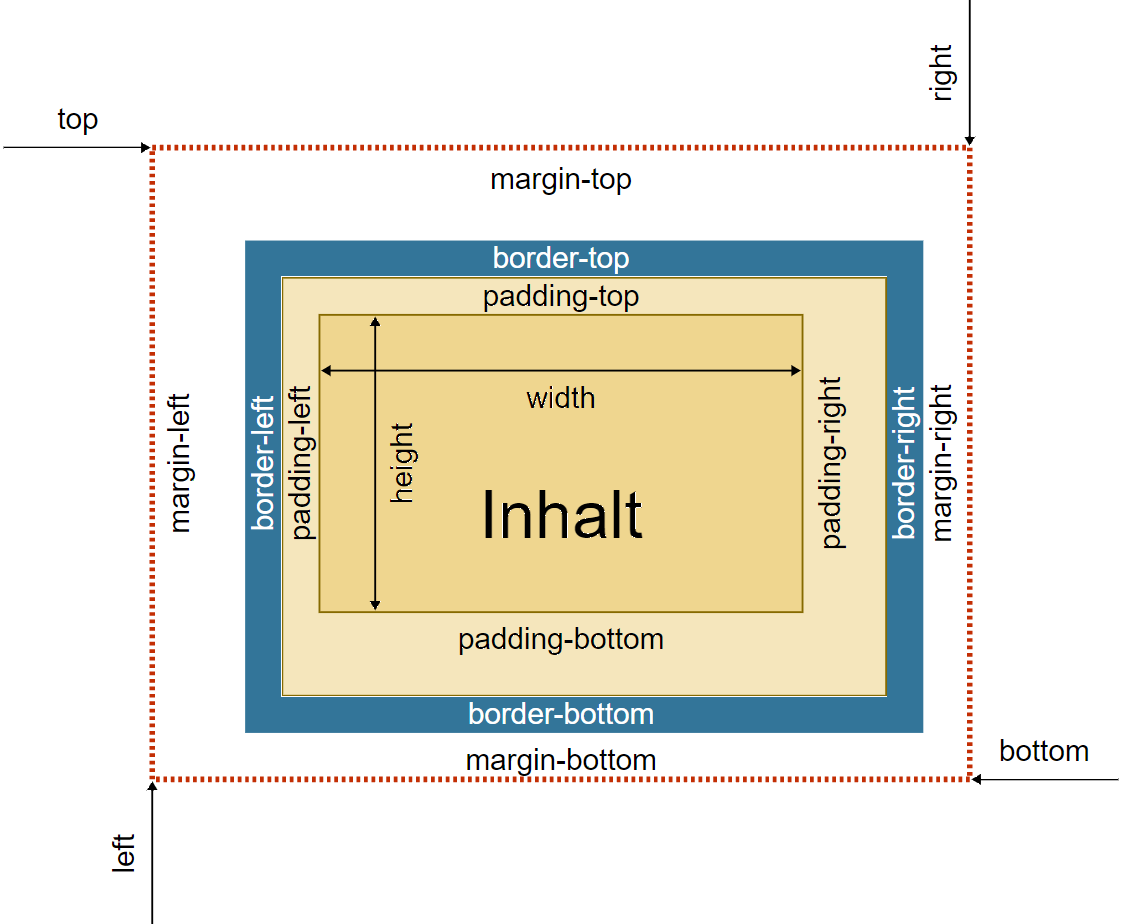
\includegraphics[width=0.75\textwidth]{includes/figures/bonus_css_position.png}
    \end{center}
\end{bonus}

\begin{bonus}{Flexbox}
    Eine \emph{Flexbox} verzichtet auf feste Breiten, wobei sich das flexible Element an den tatsächlich verfügbaren Platz anpasst, indem es die Leerräume zwischen den Elementen gleichmäßig verteilt.
\end{bonus}

\begin{bonus}{Bootstrap}
    Responsive Design wird zumeist mittels Frameworks erreicht.

    \emph{Bootstrap} ist das populärste CSS-Framework und verfolgt einen Mobile-First-Ansatz.
    Die Layout-Stile wurden zunächst für kleine Bildschirme entworfen, um sie dann den größeren anzupassen.

    Bootstrap wird wie CSS im Head-Element zumeist von einem externen Anbieter (CDN) eingebunden:
    \begin{lstlisting}[language=HTML5]
        <link rel="stylesheet" 
            href="https://maxcdn.bootstrapcdn.com/bootstrap/3.3.7/css/bootstrap.min.css">
    \end{lstlisting}
\end{bonus}